\documentclass[10pt,conference,compsocconf]{IEEEtran}

\usepackage{hyperref}
\usepackage{graphicx}	% For figure environment
\usepackage{todonotes}
\usepackage{cleveref}


\begin{document}
\title{Comparing Optimizers: Studying the Impact of Lion and Other Optimizers on Model Generalization}


\author{
  Nicolas Bonnefoy (366937), Oliver Dudler (367451), Nicolas Pellerin (367388)\\
  \textit{Optimization for Machine Learning - CS-439, EPFL Lausanne}
}

\maketitle

\begin{abstract}

  This study compares the Lion optimizer, a novel optimization algorithm, with other well-known optimizers to evaluate its performance in training neural networks. Using the CIFAR-100 dataset and the ResNet18 and ResNet101 models, we investigate the impact of the choice of optimizer on accuracy and generalization. Our experiments, conducted with limited resources using budgeted training, reveal that the Lion optimizer outperforms other optimizers, achieving higher accuracy and lower generalization error. These results confirm the superior performance of the Lion optimizer reported in previous studies. Additionally, our findings highlight the significance of selecting an appropriate optimizer, as the choice of optimizer does influence the model's generalization ability.

\end{abstract}

\section{Introduction}
Optimizers are a key component of the machine learning process. Although many different optimizers exist, one of them has been dominating since 2014: ADAM. Very recently, a new optimizer called LION has emerged as a serious challenger to Adam supremacy \cite{lion} (Evo\textbf{L}ved S\textbf{i}gn M\textbf{o}me\textbf{n}tum). In this mini-project, we empirically compare the performances of this new Lion optimizer with the performances of other well-known optimizers. The creator of the Lion optimizer have shown that it performs better than other usual optimizers on a variety of networks/tasks \cite{lion}. We aim to check if that edge in performance still holds when training on a relatively tight computing budget. More specifically, we study to what extent the choice of the optimizer affects the models generalization capacities. We therefore explore the performances of the Lion optimizer in the early stages of training and the generalization power that follows such a budgeted training.

The entire project code and the presented results can be viewed on our GitHub repository \cite{github}

\section{Models and Methods}
\subsection{Dataset}
We train and test on the CIFAR-100 \cite{cifar100} dataset. The CIFAR-100 dataset consists of $60 000$ $32$x$32$ color images pertaining to $100$ different classes. Each class contains $600$ images. The dataset is split into a training set of $50'000$ images and a test set of $10'000$ images. We chose the CIFAR-100 dataset due to its challenging nature. It provides a solid testing ground for the evaluation and comparison of different optimizers performances.

\subsection{Model}
We train and test both ResNet18 and ResNet101 models. These two models are convolutional neural networks used for computer vision tasks such as image recognition and image classification. They are composed of $18$ and $101$ convolution layers respectively and use residual connections as their name suggests. We use the implementation of the models made available by the \verb+PyTorch+ package.

\subsection{Optimizers}
We selected a total of five optimizers for comparison \cite{optimizers}:
\begin{enumerate}
  \item SGD (Stochastic Gradient Descent): It updates the model's parameters by moving in the direction of the negative gradient of the loss function, using a fixed learning rate.
  \item SGDM  (Stochastic Gradient Descent with Momentum): It enhances SGD by adding a momentum term that accumulates past gradients to accelerate learning, helping to overcome local minima and plateaus.
  \item RMSProp or RMS (Root Mean Square Propagation): It adapts the learning rate for each parameter based on the magnitude of recent gradients. It divides the learning rate by an exponentially decaying average of squared gradients, which reduces the impact of large gradient updates.
  \item ADAM  (Adaptive Moment Estimation): It combines the benefits of momentum and RMSprop. It maintains an exponentially decaying average of past gradients and squared gradients, and uses bias correction to estimate the first and second moments of the gradients. It provides adaptive learning rates for each parameter.
  \item LION: It is a recent optimizer that uses symbolic regression to automatically discover optimization algorithms tailored for a specific problem.
\end{enumerate}


We train each of the above-mentioned models with each optimizer on the selected dataset. We use the implementations of the optimization algorithms provided by the \verb+PyTorch+ package.

\subsection{Methods}
Through the training procedure, the model parameters are modified by the optimizer in order to decrease the loss function. We used the cross-entropy loss with 100 classes. For each model and each optimizer, we ran a grid-search to find the best hyperparameters we could for the training. Our goal was to compare the different optimizer's performance at their best. The grid-search was two-fold. First, we skimmed through the literature \cite{hyperp1}, \cite{hyperp2}, \cite{hyperp3} to find well-performing values for our selected models and task. We used these as a baseline to perform a coarse-grained grid-search in an already restricted yet sound hyperparameter space. Then, we performed a more fine-grained search around the values found in the first search. \Cref{hyperparams} reveals the best hyperparameters we found for each pair of model and optimizer. A dash (\verb+-+) denotes that the specific hyperparameter is not used by that optimizer.

\begin{table}[htbp]
  \centering
  \caption{Results of the two-step Grid Search}
  \begin{tabular}[c]{|l|l||l|l|l|}
    \hline
    Model     & Optimizer & Learning Rate & Weight Decay & Momentum \\
    \hline
    ResNet18  & SGD       & $0.01$        & $0.005$      & $-$      \\
    ResNet18  & SGDM      & $0.01$        & $0.005$      & $0.9$    \\
    ResNet18  & RMS       & $0.0001$      & $1$e-$05$    & $0.9$    \\
    ResNet18  & Adam      & $0.0003$      & $0.1$        & $-$      \\
    ResNet18  & Lion      & $0.0003$      & $1.0$        & $-$      \\
    ResNet101 & SGD       & $0.01$        & $0.05$       & $-$      \\
    ResNet101 & SGDM      & $0.01$        & $0.005$      & $0.9$    \\
    ResNet101 & RMS       & $1$e-$05$     & $1$e-$06$    & $0.95$   \\
    ResNet101 & Adam      & $9.5$e-$05$   & $0.05$       & $-$      \\
    ResNet101 & Lion      & $7$e-$05$     & $1.0$        & $-$      \\
    \hline
  \end{tabular}
  \label{hyperparams}
\end{table}

Initially, for the hyperparameter tuning, we wanted to use 5-fold cross-validation. However, due to limited resources, we had to compromise and use a single validation set instead, composed of $20$\% of the available training data.

We use budgeted training and only trained the models for a total of $10$ epochs, we choose this number of epochs in order to obtain clear results but stay in a budgeted training situation. We used a training batch size of $256$ to strike a balance between computational efficiency and model stability, and a test batch size of $1000$ as it allows multiple examples of each class to be used during the test and makes it representative enough.

\section{Results}
Using the hyperparameters illustrated in \Cref{hyperparams} we trained each of the two models with all five selected optimizers and obtained the following results.

\begin{figure}[htbp]
  \centering
  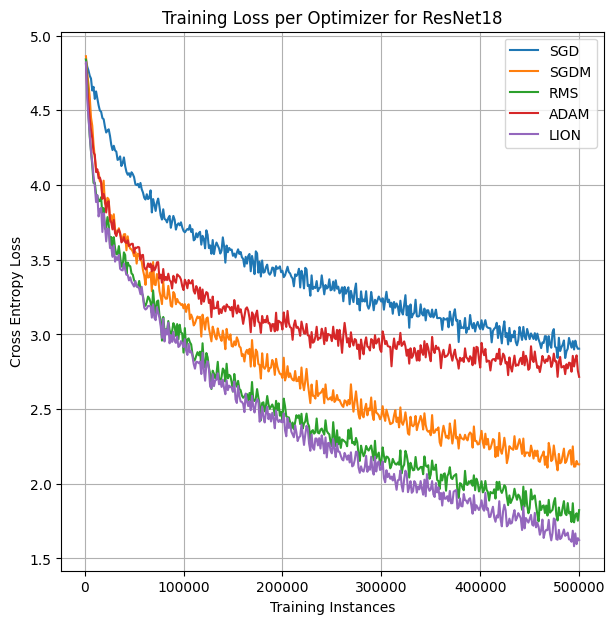
\includegraphics[width=0.8\columnwidth]{train_loss_18}
  \caption{Training Loss per Optimizer for the ResNet18 Model}
  \vspace{-3mm}
  \label{train_loss_18}
\end{figure}

\Cref{train_loss_18} shows the training loss achieved by ResNet18 per optimizer. We can see that as expected LION performs the best, and that already after a few epochs when compared to SGD, SGDM, or ADAM. RMS has very close results and the gap appears only after half the training is done. SGD and ADAM seem to reach a plateau fairly early during the training.

\begin{figure}[htbp]
  \centering
  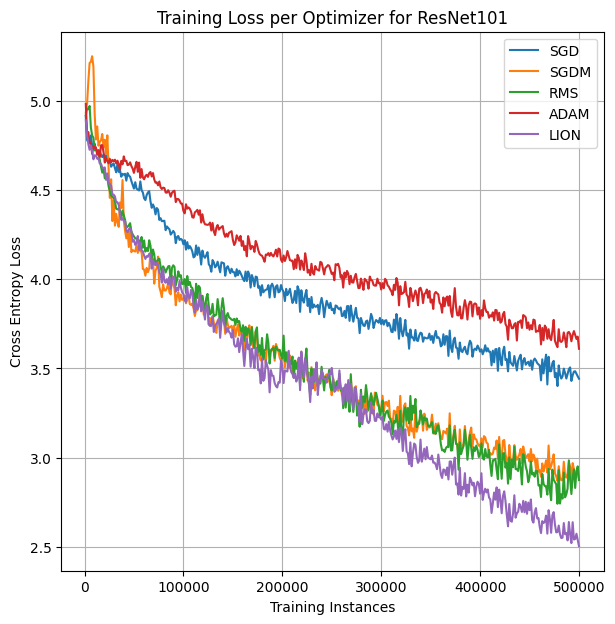
\includegraphics[width=0.8\columnwidth]{train_loss_101}
  \caption{Training Loss per Optimizer for the ResNet101 Model}
  \vspace{-3mm}
  \label{train_loss_101}
\end{figure}

\Cref{train_loss_101} shows the training loss achieved by ResNet101 per optimizer. Here again, we observe that LION performs the best, taking an early lead on SGD and ADAM. A few epochs before the end of the training, RMS and SGDM's progression starts to slow down and LION starts to have a clear advantage.

\begin{figure}[htbp]
  \centering
  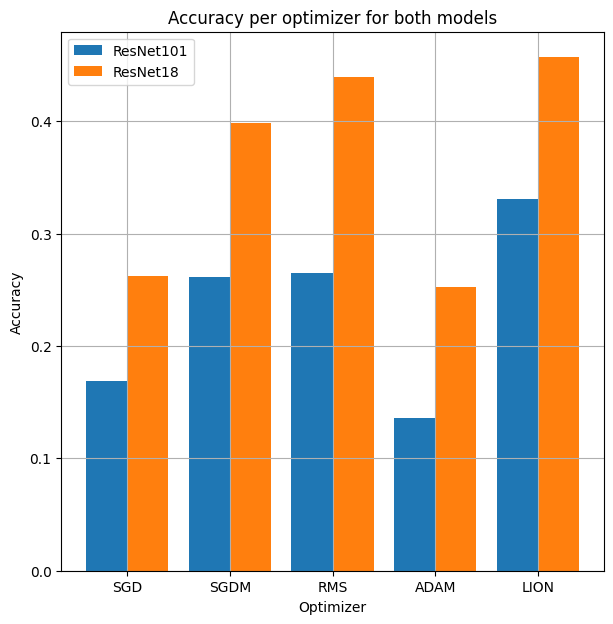
\includegraphics[width=0.8\columnwidth]{acc}
  \caption{Achieved Accuracy per Model and per Optimizer}
  \vspace{-3mm}
  \label{acc}
\end{figure}

\Cref{acc} shows the accuracy achieved by the ResNet18 and ResNet101 per optimizer. In our experiments, LION outperforms the four other optimizers on both models. We notice that RMS achieves the second-best results, those being fairly close to the results of LION, and also that ADAM performs very poorly with both models.

\begin{figure}[htbp]
  \centering
  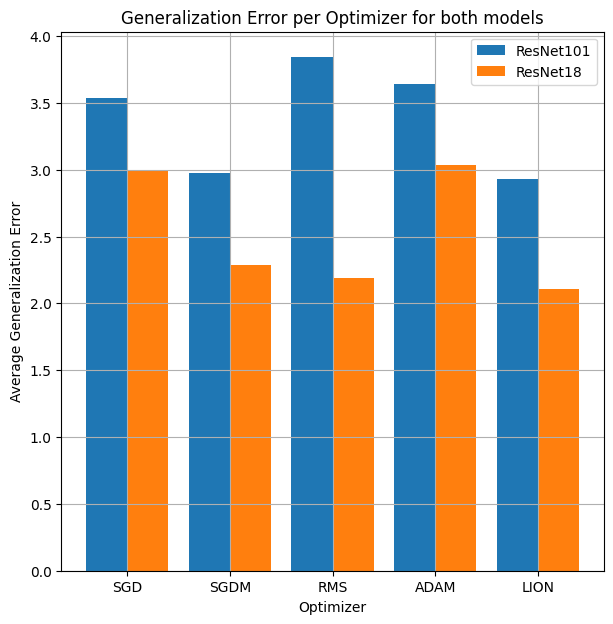
\includegraphics[width=0.8\columnwidth]{gen}
  \caption{Generalization Error per Model and per Optimizer}
  \vspace{-3mm}
  \label{gen}
\end{figure}

\Cref{gen} shows the generalization error over the test set per model and per optimizer. Finally, it appears again that LION manages the best results, and this time SGDM gets the second-best results.

\section{Discussion}
Our experiments show that the Lion optimizer consistently outperforms the other optimizers. After training for $10$ epochs, the lion optimizer gave the best accuracy for both models ($45.7$\% and $33.0$\%) and the lowest generalization (test) error. These results align with Lion birth-study \cite{lion-study} and highlight the importance of selecting an appropriate optimizer for training neural networks. 

Regarding the relationship between the training loss and generalization (test) error, the hierarchy between optimizers is sometimes reversed in our experiments. For example with ResNet18, ADAM finishes training the model to a lower loss than what SGD was able to. However when it comes to the test error, the hierarchy is reversed: the model trained with SGD i.e. with the higher loss, gets a better test score than the model trained with ADAM i.e. with the lower loss. 

The superior performance of the Lion optimizer, even with limited training resources and a budgeted training approach, underscores its effectiveness in optimizing model performance. An even more comprehensive hyperparameter search could potentially improve the performance of some of the other optimizers but shouldn't change results. 


\section{Extensions}

Reflecting on our work, it is possible that our training was indeed too budgeted. Adam performed suspiciously poorly although it has been the king of optimizers for almost a decade. Maybe our experiments could be expanded for a bit more epochs to see if Lion early dominance still prevails. It could also be interesting to extend this study to different tasks or models such as VGG for instance.

\section{Summary}
While we were aware that Lion outperforms other optimizers in full-training settings, we wondered how it would perform when the compute budget is restricted. In our experiments, Lion did maintain its superiority on the CIFAR-100 dataset with both ResNet-18 and rest-net101. In terms of loss, Lion was able to lower it down the fastest. However, we were interested in how well models would generalize when trained for such little time. Again, both ResNet models had their highest generalization capabilities when trained with Lion. So as far as our experiments go, we can declare Lion the winner of this training competition.


\bibliographystyle{IEEEtran}
\bibliography{literature}

\end{document}
